\documentclass[10pt]{article}

\usepackage{mathtools}  % need for math tools
\usepackage{amsmath}    % need for subequations
\usepackage{graphicx}   % need for figures
\usepackage{verbatim}   % useful for program listings
\usepackage{color}      % use if color is used in text
\usepackage{subfigure}  % use for side-by-side figures
\usepackage{hyperref}   % use for hypertext links, including those to external documents and URLs


\setlength{\baselineskip}{16.0pt}   
\setlength{\parskip}{3pt plus 2pt}
\setlength{\parindent}{20pt}
\setlength{\oddsidemargin}{0.5cm}
\setlength{\evensidemargin}{0.5cm}
\setlength{\marginparsep}{0.75cm}
\setlength{\marginparwidth}{2.5cm}
\setlength{\marginparpush}{1.0cm}
\setlength{\textwidth}{150mm}

\begin{document}

\begin{center}
{\large Ay190: Computational Astrophysics (Winter Term 2012)} \\
{\large HomeWork - 7 } \\
\copyright 2012 by Arya Farahi \\
Feb 25, 2012
\end{center}

\section{Exercise 1. Building a 1D planar Finite-Volume Hydrodynamics Code}


\begin{figure}[hbt]
  \begin{center}
    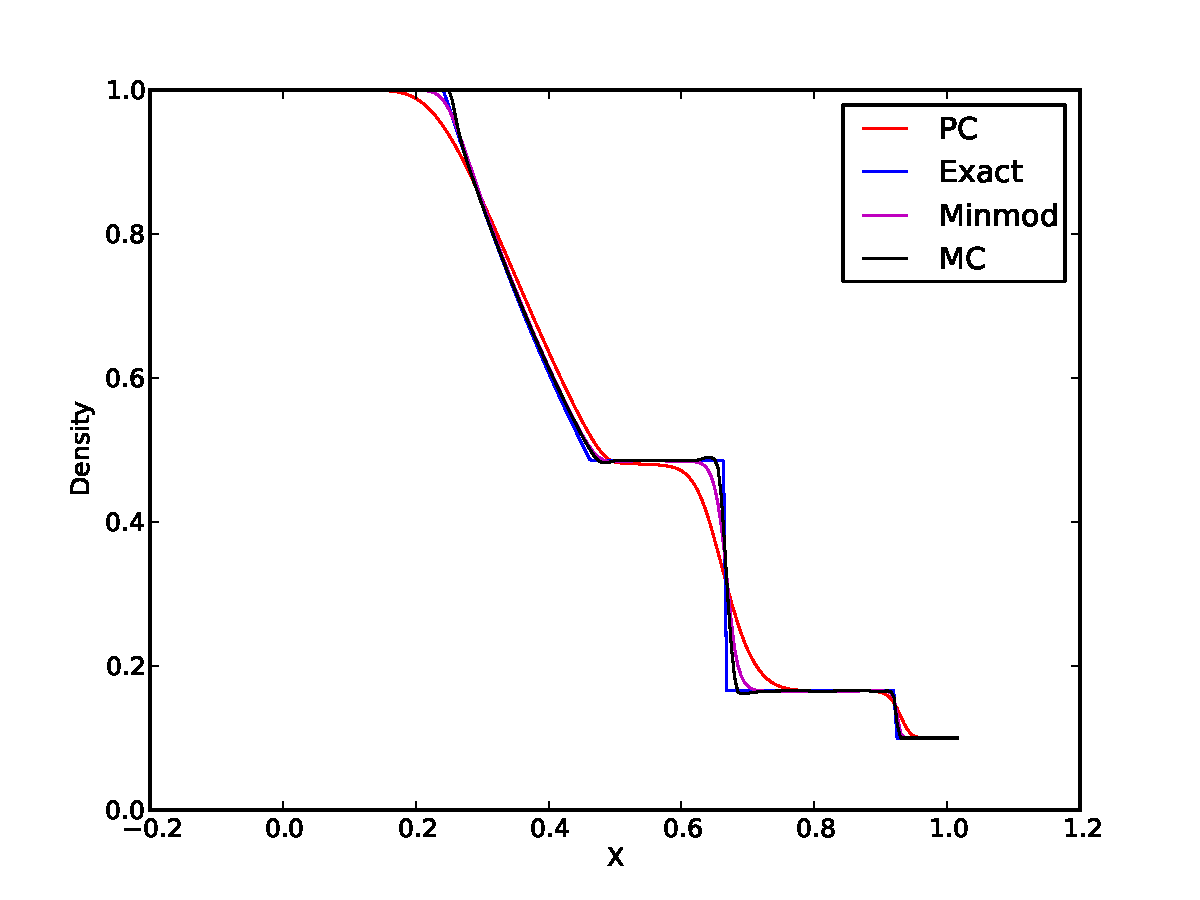
\includegraphics[scale=0.4]{Plots/plot1.pdf}
    \caption{\label{fig:1} Plot of the solution of riemann problem with PC, Minmod, and MC method + exact solution.}
  \end{center}
\end{figure}

\begin{figure}[hbt]
  \begin{center}
    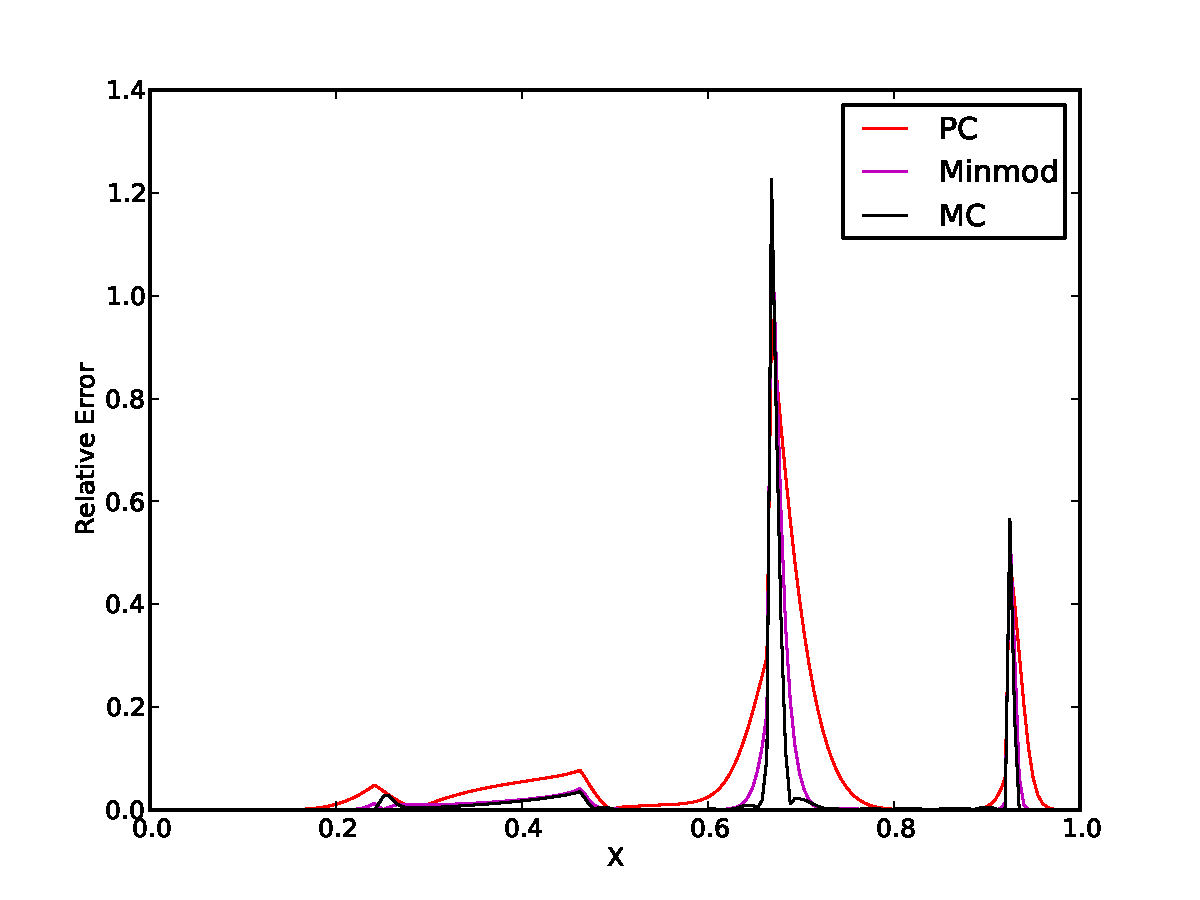
\includegraphics[scale=0.4]{Plots/plot2.pdf}
    \caption{\label{fig:2} Plot of the relative error of PC, Minmod, and MC methods.}
  \end{center}
\end{figure}

Figure \ref{fig:1} shows solution of riemann problem with PC, Minmod, and MC method with compare to the exact solution, and \ref{fig:2} shows the relative error of PC, Minmod, and MC method. It shows that MC method is the best one and then Minmod is the good one and the PC method is the worst. \\

It seems that for this specific problem MC method is much more better than the other ones, because first of all it converge to real answer much more faster than the other one. \\ 

\pagebreak




\end{document}
